

\section{Head aesthetic design} % (fold)

Lot of effort have been put in the design and aesthetic of Poppy's head (see \figurename~\ref{fig:poppy_beta_head}), both its identity and main communication apparatus.
On an aesthetic point of view, its design was inspired of course by existant robots, but also by animals, objects and arts. The main inspiration insight are displayed as a board on the \figurename~\ref{fig:head_inspiration}. We tried to make to achieve a design cute, expressive and among all simple.

\begin{figure}[p]
    \begin{center}
        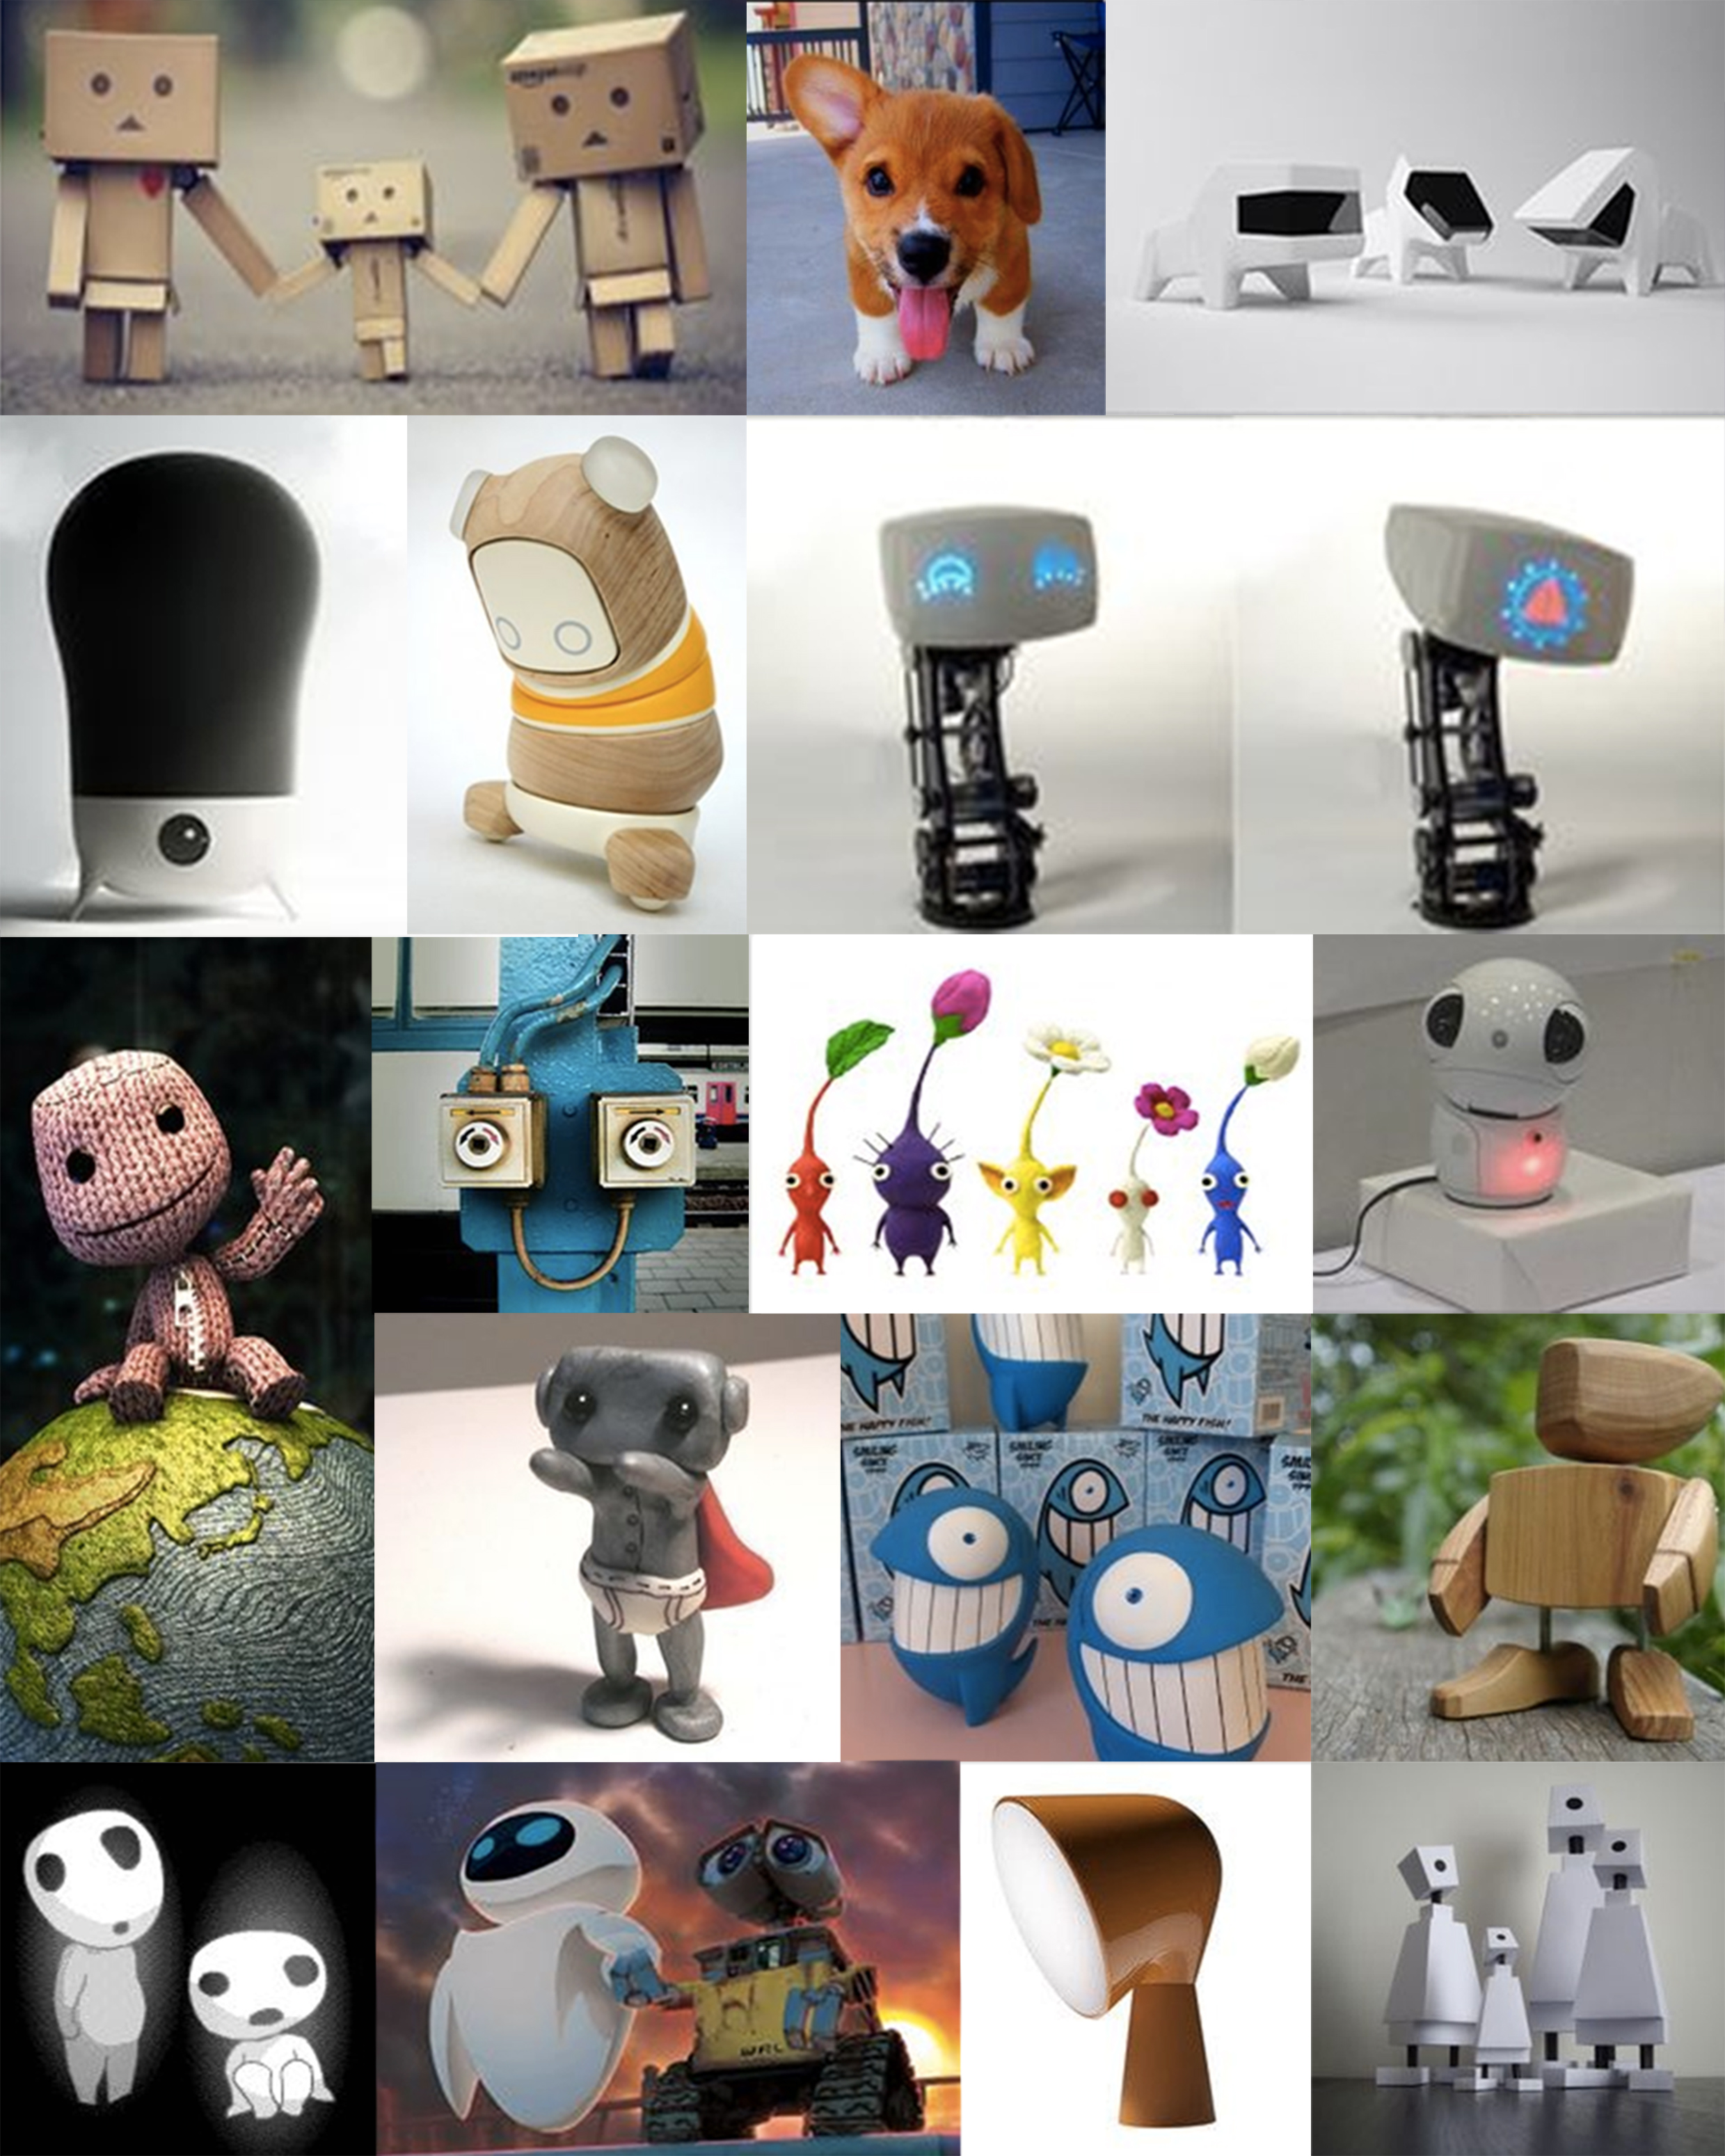
\includegraphics[width=\linewidth]{head_inspiration.jpg}
    \end{center}
    \caption{Complete board available on pinterest \url{http://www.pinterest.com/matthieulapeyre/robot/}}
    \label{fig:head_inspiration}
\end{figure}

Yet because of the multi-articulated vertebral column, Poppy has only free room in the head to embed all electronics components needed. Therefore strong technical constraints were imposed because the head has to embed all electronic architecture plus the communication sensorimotor apparatus composed by a wide 4.3" screen, cameras, audio.
This components strongly constraints the design of the robot. Especially the screen, which requires a large flat part on the face. Obtaining a nice and rounded head shape with such constraints were rather difficult and require several iterations before obtaining a first correct finish (see \figurename~\ref{fig:poppy_beta_head}).

% This process involved first few sketches that gave the main idea of the desired design. Yet the transfer to CAD modeling was quite complex, this kind of shape are rather difficult to design using parametric tools.

\begin{figure}[p]
\centering
    \subfloat[][]{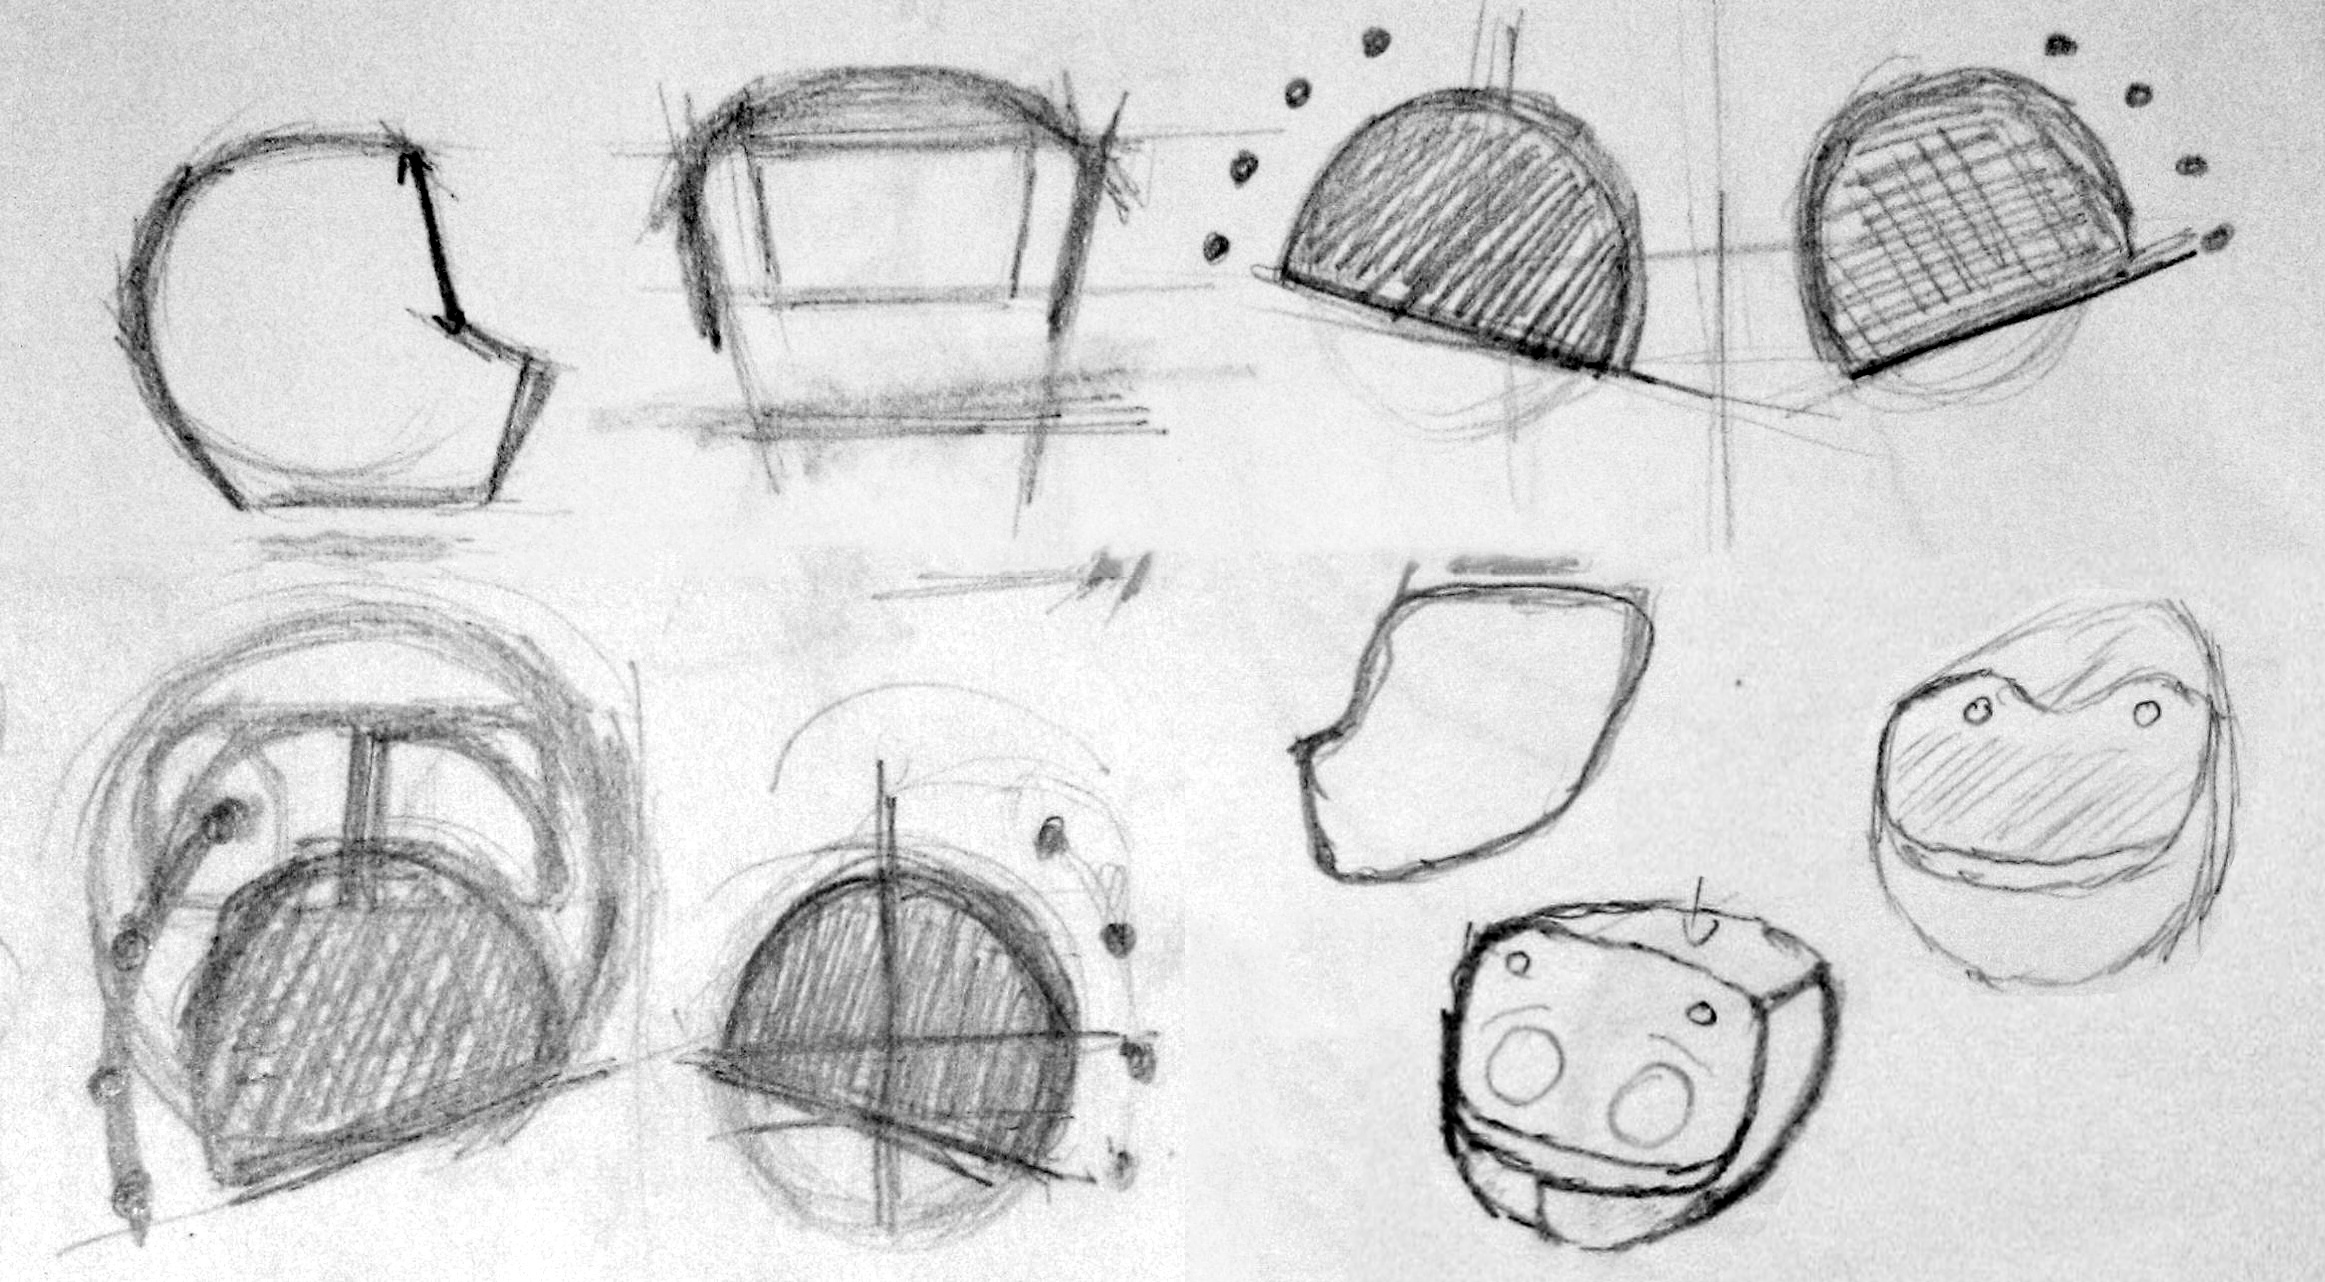
\includegraphics[height=4.5cm]{first_sketch.jpg}}
    \hfil
    \subfloat[][]{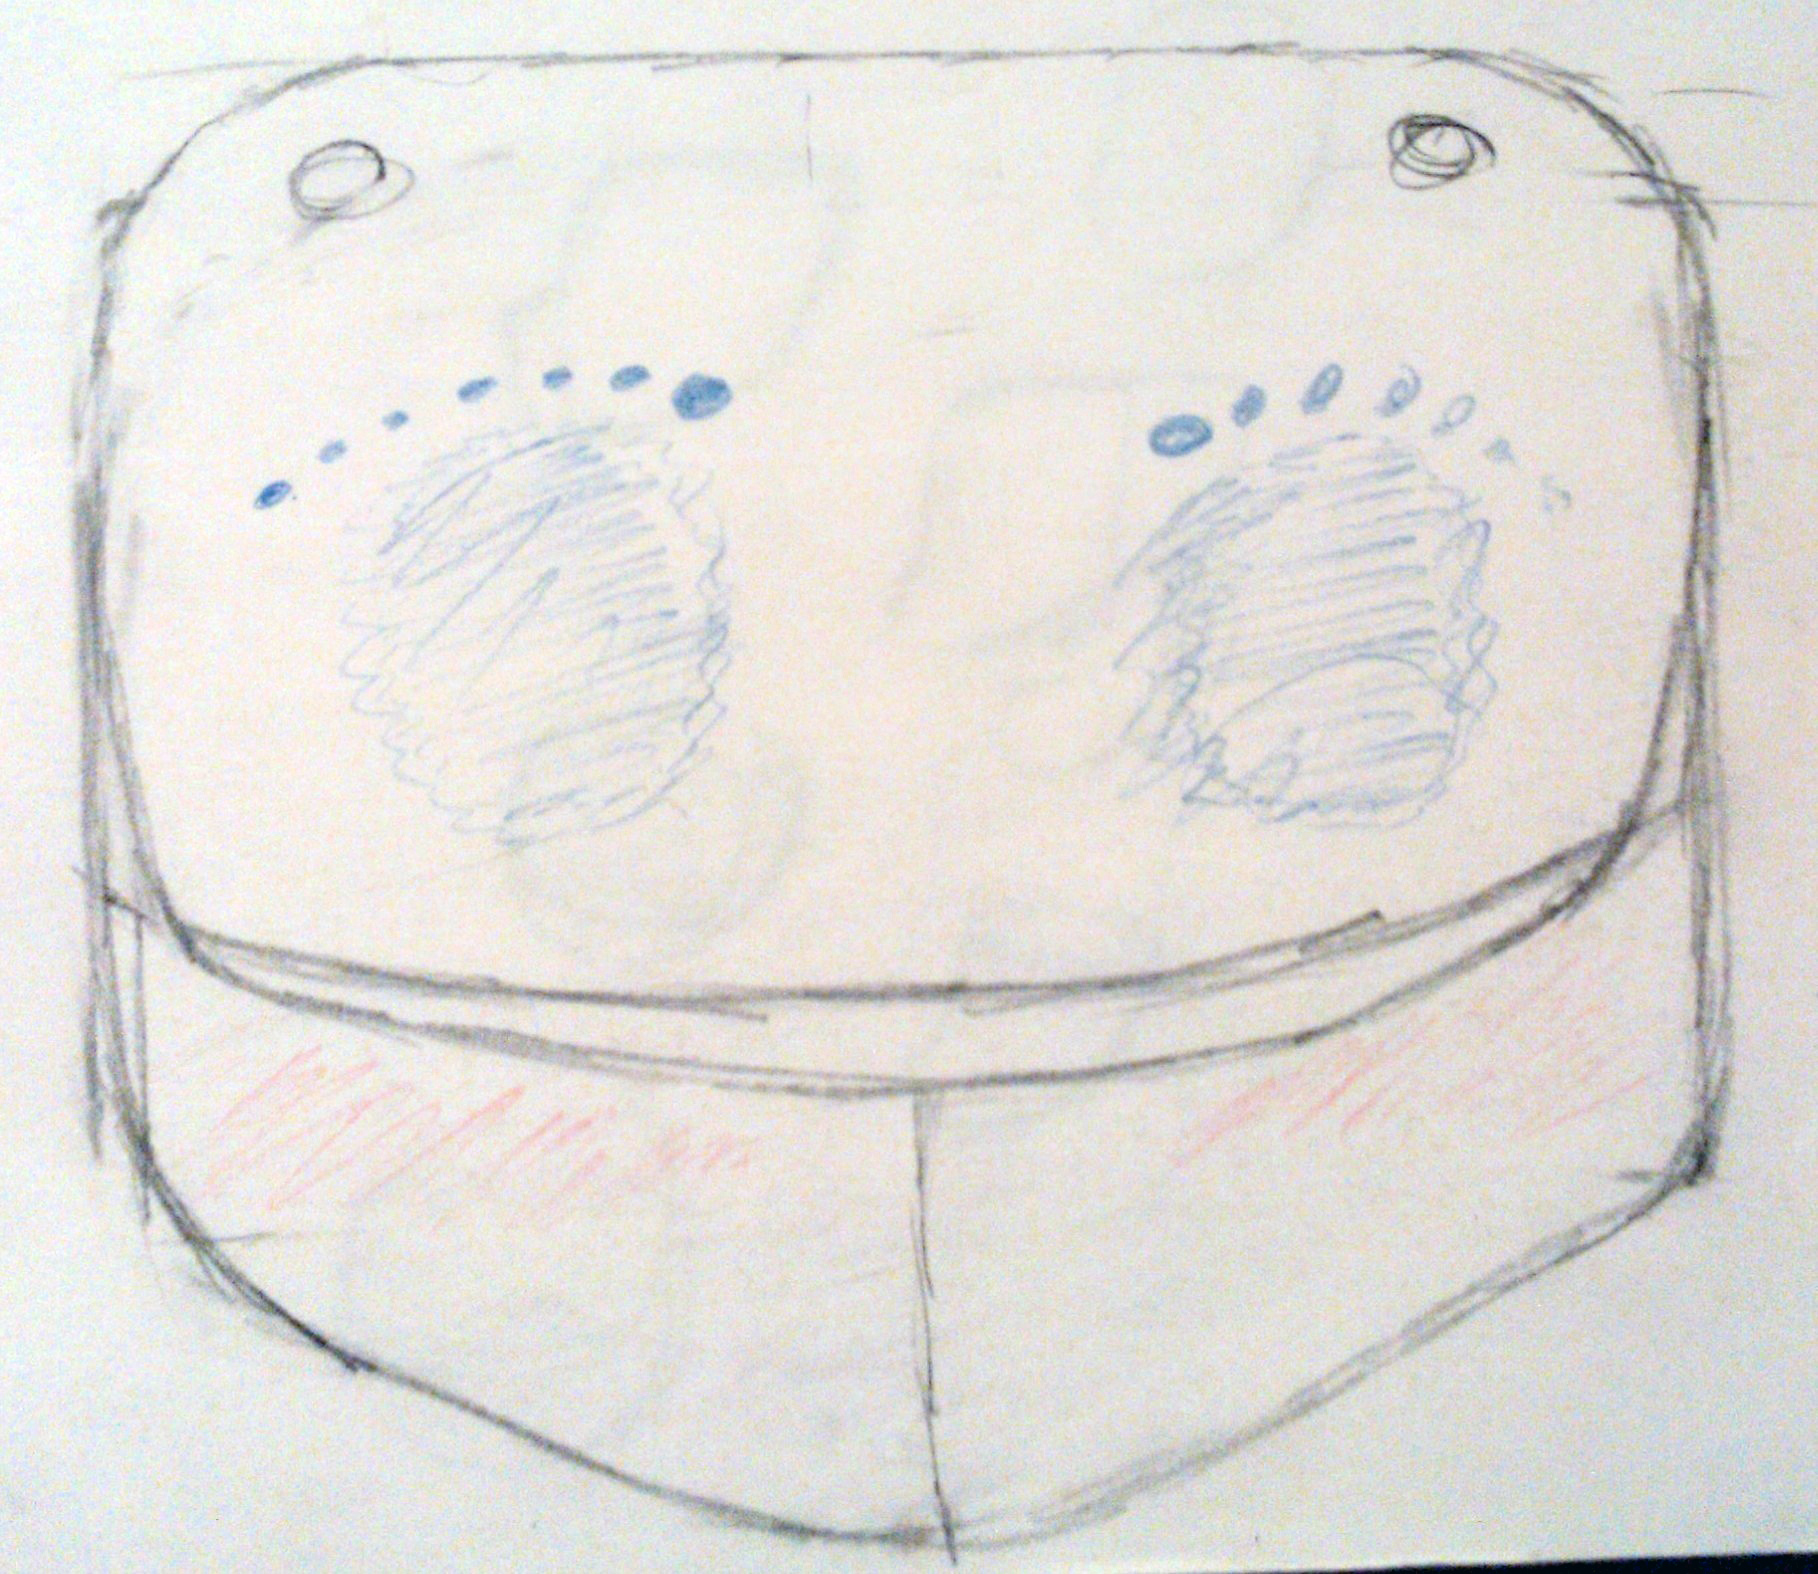
\includegraphics[height=4.5cm]{poppy_head_sketch.jpg}}
    \newline
    \subfloat[][First clay sculpture]{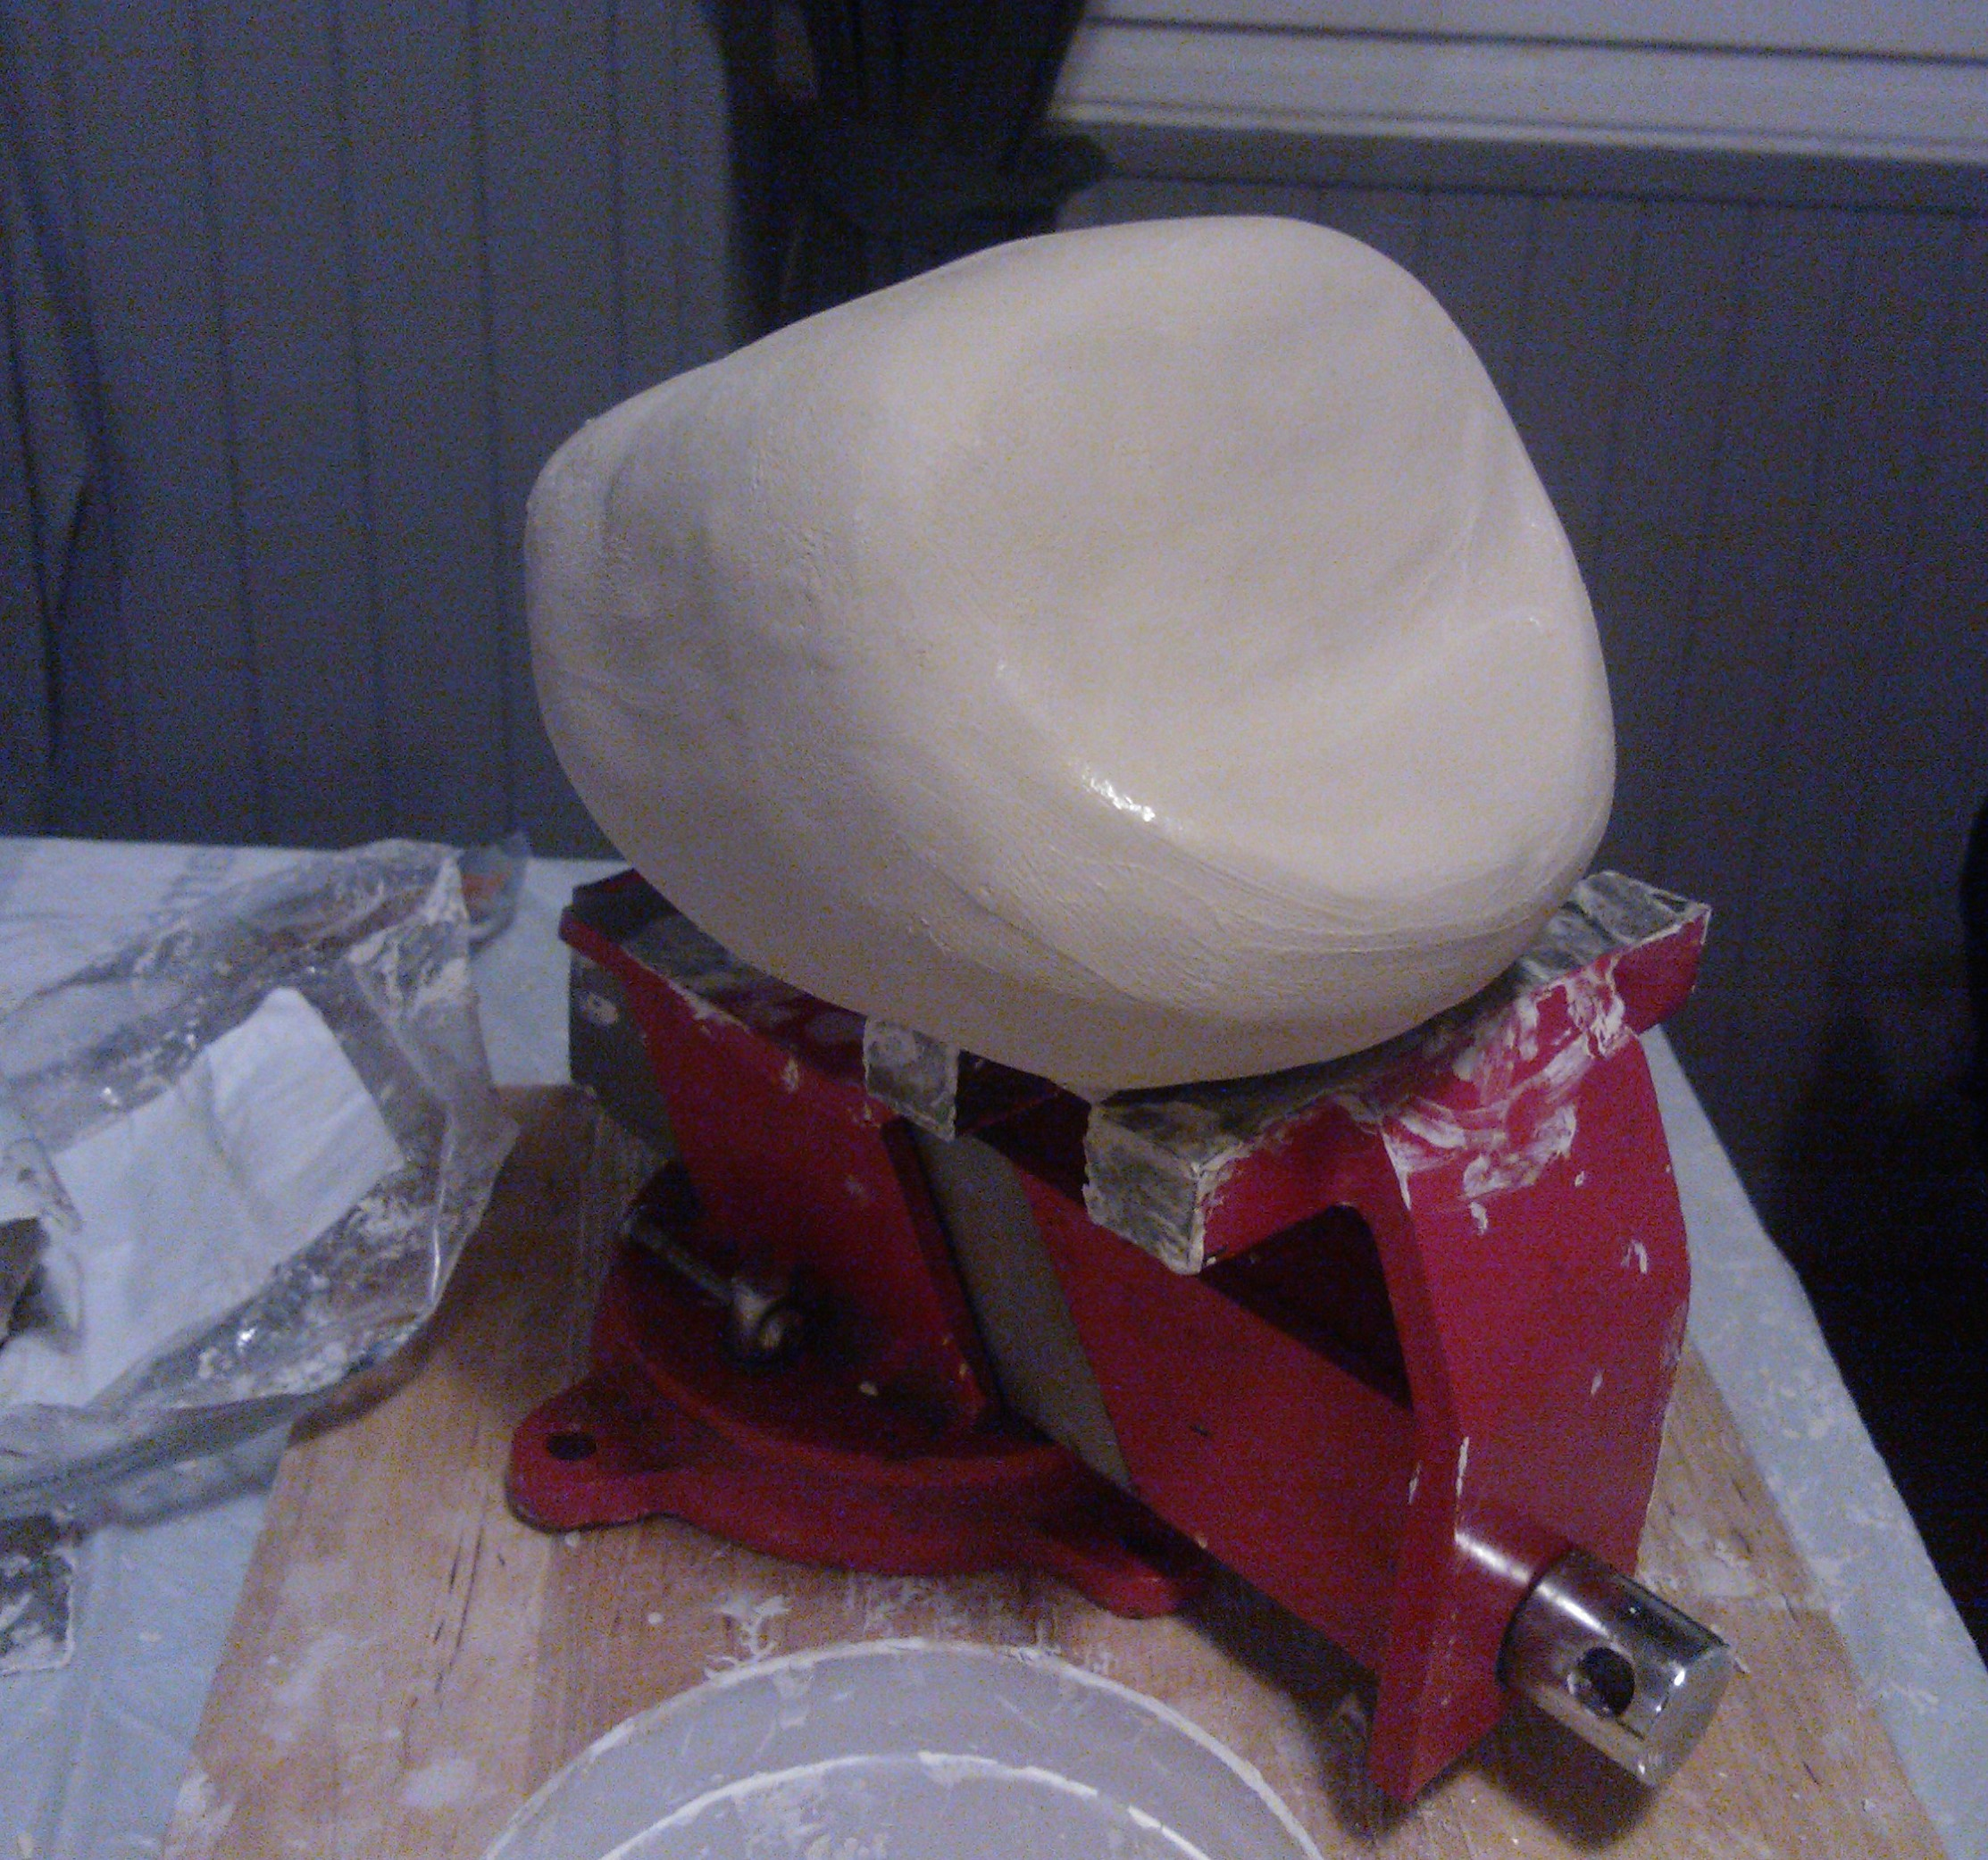
\includegraphics[height=5.5cm]{first_poppy_clay.jpg}}
    \hfil
    \subfloat[][First CAO model]{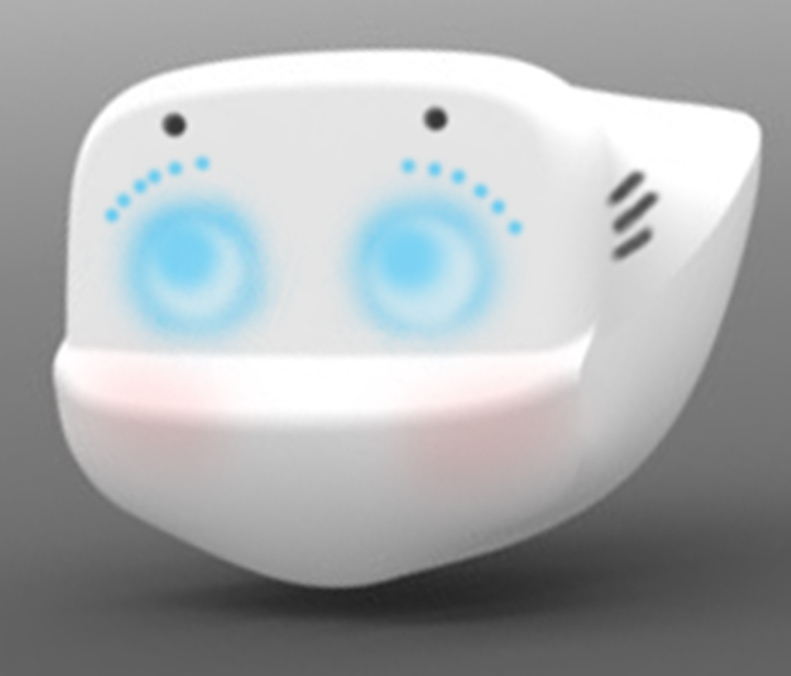
\includegraphics[height=5.5cm]{head_first_trial.jpg}}
    \newline
    \subfloat[][Poppy beta]{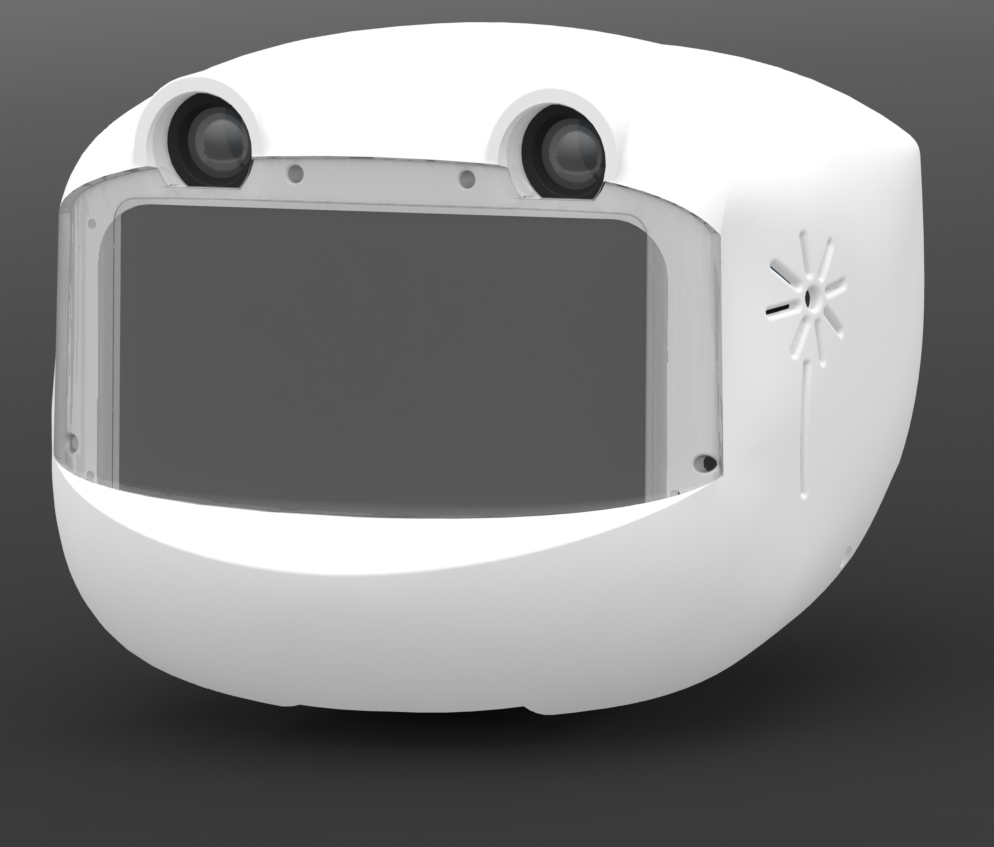
\includegraphics[height=5.5cm]{head_beta.jpg}}
    \hfil
    % \subfloat[][The first assembly]{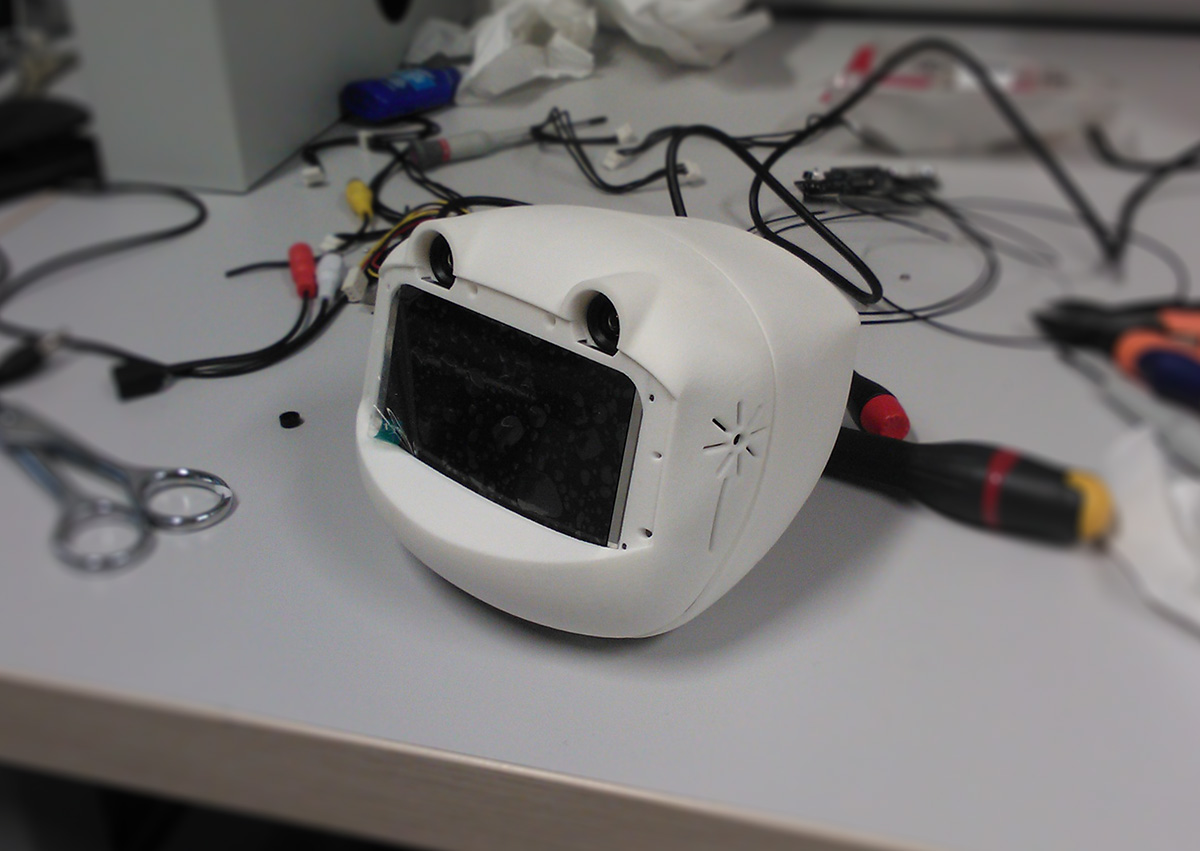
\includegraphics[height=5.5cm]{head_beta_assembled.jpg}}
    % \hfil
    \subfloat[][Screen powered on with basic eyes display]{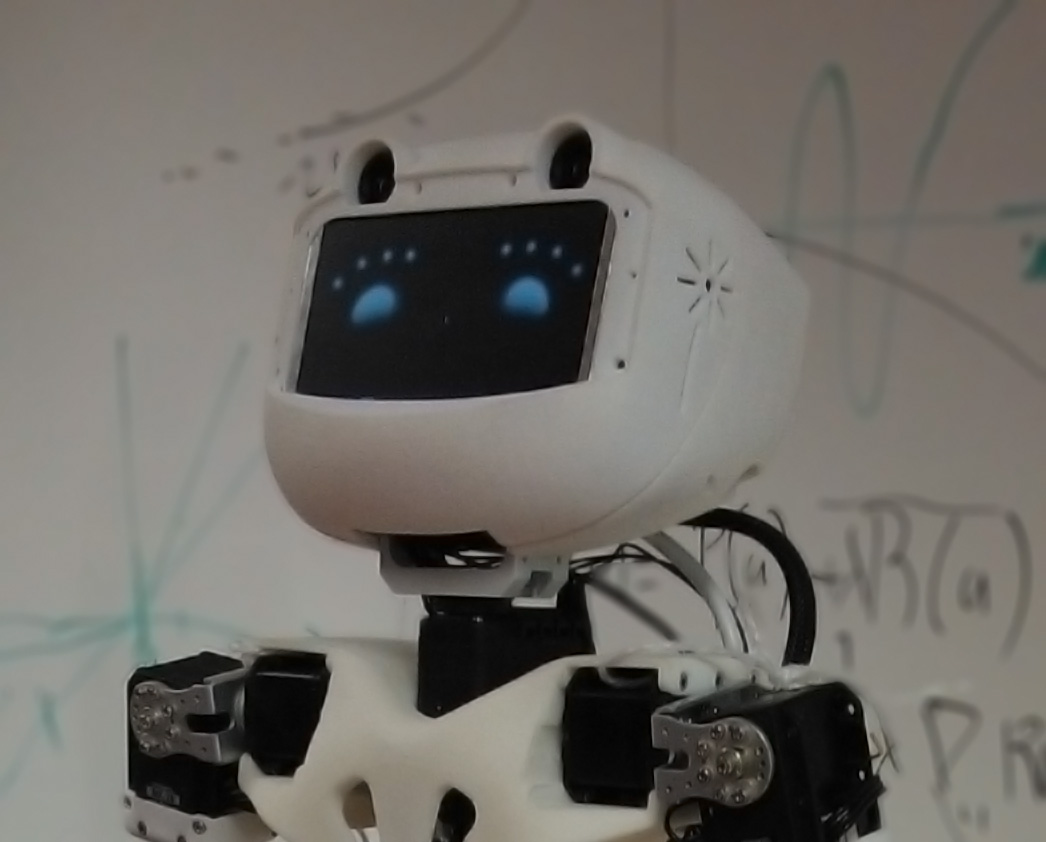
\includegraphics[height=5.5cm]{poppy_beta_eyes.jpg}}
    \caption{Evolution of Poppy head from the first sketches to the Poppy beta version.}
    \label{fig:head_sketch}
\end{figure}


However, in the first beta version showed here, there is a major design error. Indeed my desire was to have a screen to create and explore freely expressive eyes but the use of two visible cameras changed the way people saw Poppy's head. Of course, people seeing 2 cameras considers they are the eyes of the robot and therefore extrapolate that the screen may be the mouth.

We are working on this issue by replacing the two big camera by a small one with a pinhole lens, which can be hidden on the Poppy face see \figurename~\ref{fig:poppy_head_v1}.

\begin{figure}[tb]
\centering
    % \subfloat[][Mix between Poppy beta 3D printed head and clay sculpture]{\includegraphics[height=5cm]{second_poppy_clay.jpg}}
    % \newline
    \subfloat[][Poppy 1.0]{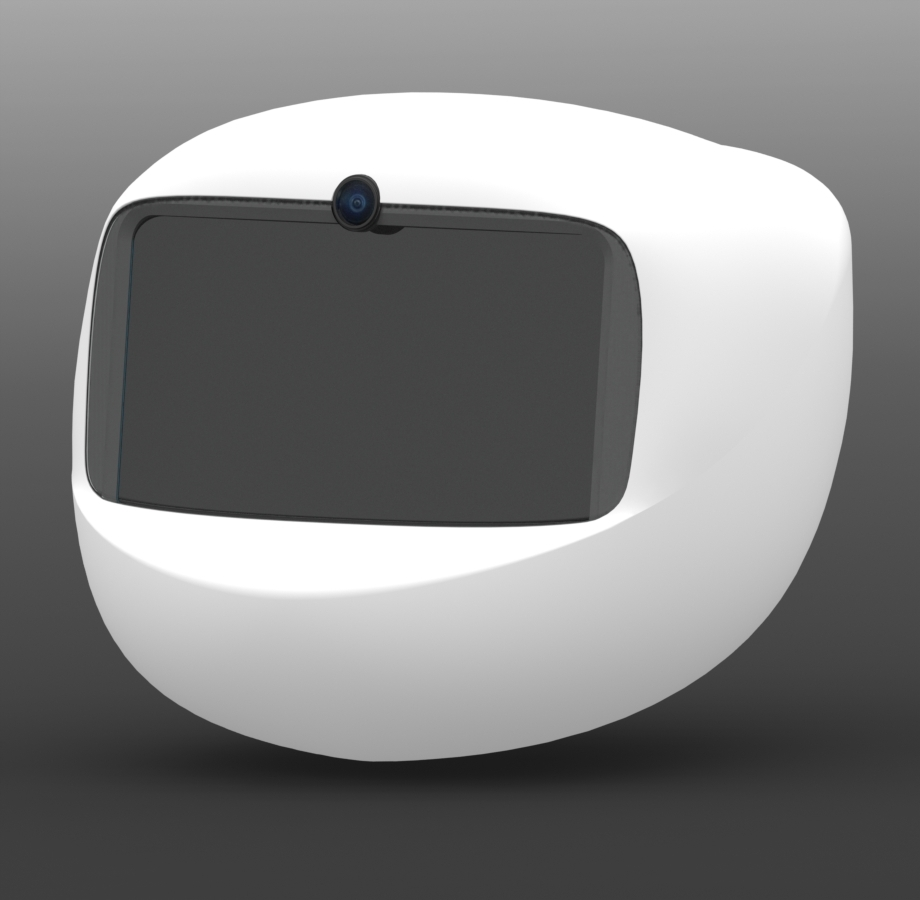
\includegraphics[width=0.5\linewidth]{poppy_v1_head.jpg}}
    \caption{}
    \label{fig:poppy_head_v1}
\end{figure}
